\chapter{Numerical Studies}
Having discussed how the NSE were simplified, discretized, and implemented, in this section the implementation is tested and validated.
To this end, first the results of the unit tests from section \ref{sec:testing} are discussed by looking at the numerical errors made by the differential operators and integrators.
Thereafter the implementations of the non-hydrostatic NSE discussed in section \ref{sec:non_hydrostatic} are analyzed.

\section{Validation by Analyzing Numerical Errors}
In this section the results of the tests performed in section \ref{sec:testing} are discussed.

% analysis of errors
\subsection{Differential Operators}
To test the differential operators, the function $f(x)=\sin(20\pi (x-e))$ was used on the domain $[0;1]$.
The offset of $e$ was introduced in order to avoid random perfect results.
Without it, if, for example, the samples happen to be located at the maximums, minimums and zero-crossings, even a simple central difference would make zero error.
With an offset of an irrational number, such as $e$, this is improbable.\\
For this test function the analytic result is the derivative $\frac{df}{dx}=20\pi\cos(20\pi (x-e))$.\\
To test the different methods of calculating the derivative numerically, the domain was sampled at resolutions ranging from $5$ to $20\cdot 10^7$ samples, which were spread equidistantly over the domain.\\
First, looking at the implementation of the finite differences.
If their implementation is correct, one would expect the error \texttt{finite\_ difference} $(x)-\frac{df}{dx}$ to drop with growing resolution.
More specifically for a finite difference operator of order $n$, when increasing the number of samples by a factor of $a$ one would expect a decrease in error of magnitude $a^{-n}$.
The positive result of the test can be seen in Fig. \ref{fig:derivative_error}.
\begin{figure}[!h]
	\makebox[\textwidth]{ 
  		 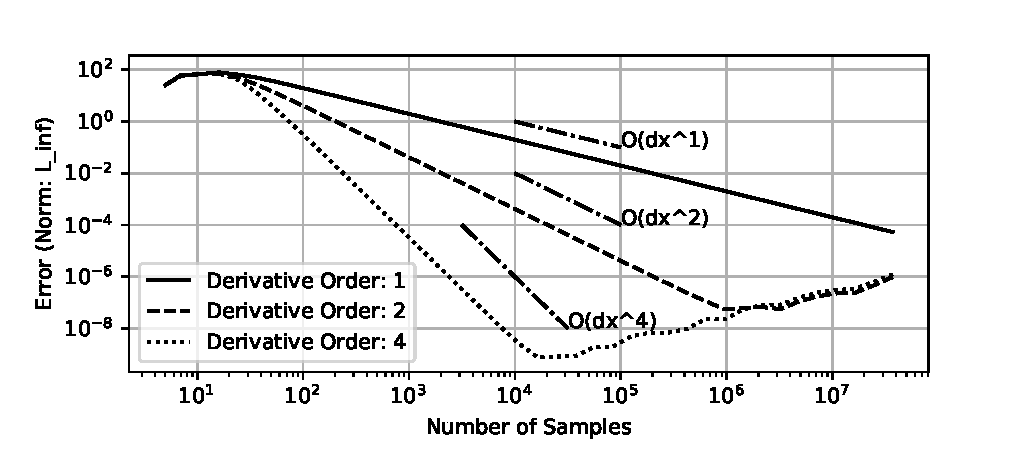
\includegraphics[width=1.2\textwidth]{figures/derivative_error.pdf}}
    \caption{Plot of error of finite difference operators over number of samples}
    \label{fig:derivative_error}
    \small
    The lines are parallel to the expected error order lines, meaning the test was successful.
\end{figure}
It can also be seen that above a certain spacial resolution, the error increases again, which is due to numerical errors.
The root of these errors is the division of a very small number in the denominator by the small number $\Delta x$, which is inversely proportional to the resolution.
This division of small numbers is not well-supported by floating point numbers, and for that reason errors will increase above a certain spacial resolution.\\
Looking at the implementation of the spectral derivative, it is expected that the error will drop down to machine precision as soon as the Nyquist sampling rate is reached.
The Nyquist sampling rate is twice the highest frequency occurring in the signal whose derivative is to be calculated.
In this case the highest frequency is $10$, because the argument of $\sin$ was $2\pi\cdot 10$, meaning the Nyquist sampling rate is $20$.
The fact this theoretical result can be observed in practice (Fig. \ref{fig:fft_error}), is a strong indication that the implementation is correct.

\begin{figure}[!h]
	\makebox[\textwidth]{ 
  		 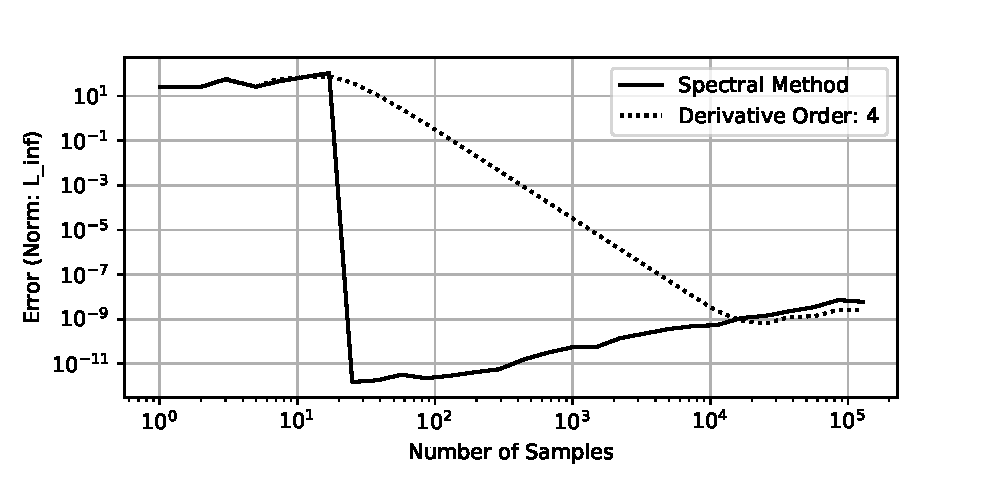
\includegraphics[width=1.2\textwidth]{figures/fft_error.pdf}}
    \caption{Plot of error of spectral derivative operator over number of samples}
    \label{fig:fft_error}
    \small
    As expected the error drops significantly as soon as the Nyquist sampling rate (20 samples) is reached.
\end{figure}

%Test-Function: $\sin(20\pi (x-e))$ on domain $[0;1]$, with resolutions from 5 to $20\cdot 10^7 $
%Actual result is $20\pi\cos(20\pi (x-e))$\\
%show how the error-order is influenced by grid-size.\\
%grid size far larger than features to be measured => inaccuracy\\
%grid size a little bit smaller than features to be measured => change in accuracy according to error-order of implemented operator\\
%grid size too small for machine precision => loss of accuracy

\subsection{Integrators}
\subsubsection{Runge-Kutta-Integrators}
As described in section \ref{sec:testing} the integrators were tested by comparing the results to analytic solution of differential equations.
Specifically, they were first tested against three types of differential equations, whose solutions are known analytically.
The first one was time-invariant and had only one variable, i.e. no spacial resolution.
The second one introduced time-variance into the mix, while the third one added spacial resolution.
In each of the tests, using a Runge-Kutta integrator of order $n$ it was expected that decreasing the time step size by a factor of $a$ would decrease the error by a factor of $a^n$.\\
\paragraph*{Time-Invariant, Single Variable}
The differential equation used is $\frac{dx}{dt}=-3x$, which has the solution $x(t)=x_0e^{-3t}$.
The result of the experiment can be seen in Fig. \ref{fig:RK_error_y'=-3y}.
\begin{figure}[!h]
	\makebox[\textwidth]{ 
  		 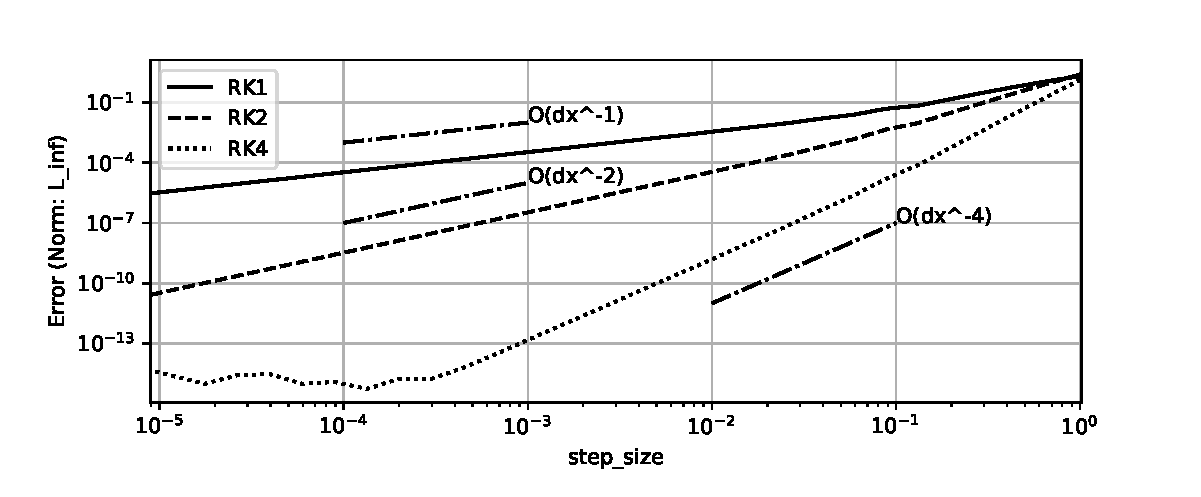
\includegraphics[width=1.2\textwidth]{figures/RK_error_y'=-3y.pdf}}
    \caption{Error of RK-methods on time-invariant, single variable differential equation}
    \label{fig:RK_error_y'=-3y}
\end{figure}

\paragraph*{Time-Variant, Single Variable}
The differential equation used is $\frac{dx}{dt}=\frac{t}{t^2+1}$, which has the solution $x_0 + 0.5\text{ln}(t^2+1)$.
The result of the experiment can be seen in Fig. \ref{fig:RK_error_y'=tdiv(t_t+1)}.
\begin{figure}[!h]
	\makebox[\textwidth]{ 
  		 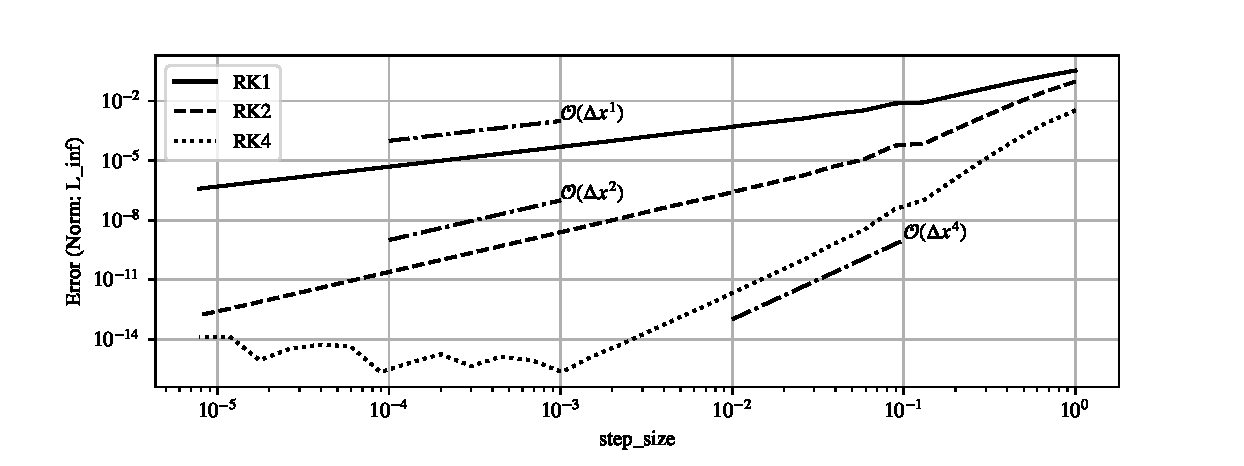
\includegraphics[width=1.2\textwidth]{figures/RK_error_y'=tdiv(t_t+1).pdf}}
    \caption{Error of RK-methods on time-variant, single variable differential equation}
    \label{fig:RK_error_y'=tdiv(t_t+1)}
\end{figure}

\paragraph*{Time-Invariant, Multiple Spatially Distributed Variables}
The differential equation used is the wave equation with periodic boundary conditions.
With $c$ being the wave propagation speed, the equation system can be written as follows:
\begin{align*}
\frac{du}{dt}&=\frac{dv}{dx}\\
\frac{dv}{dt}&=c^2\frac{du}{dx}
\end{align*}
If $u(x,t=0)=f(x)$ (with $f$ being periodic) describes the initial state of $u$, then according to d'Alembert the solution is $u(x,t)=\frac{1}{2}(f(x+ct)+f(x-ct))$, which means $v(x)=\int \frac{du}{dt} dx = \frac{c}{2}(f(x+ct)-f(x-ct))$.

\begin{figure}[!h]
	\makebox[\textwidth]{ 
  		 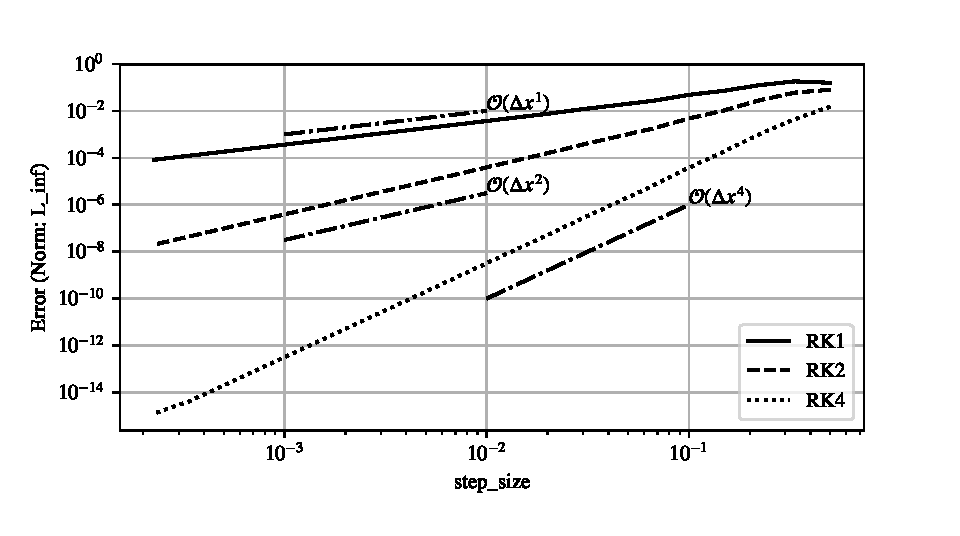
\includegraphics[width=1.2\textwidth]{figures/wave_order_line.pdf}}
    \caption{Error of RK-methods on periodic wave equation}
    \label{fig:wave_order_line}
\end{figure}

Interestingly, spacial resolution and temporal resolution are intertwined, i.e. if a very high spacial resolution (a lot of samples) is chosen, one also has to choose a high temporal resolution (small time steps).
This can be seen when plotting a heatmap of the error made when using the RK4-integrator over different spacial and temporal resolutions.
This phenomenon can be seen in Fig. \ref{fig:heatmap_wave_eq_step_size_numgridpoints}.
Roughly speaking, in order to keep the error from blowing up, an inverse proportion between spacial resolution and time step size should be kept, i.e. when doubling the spacial resolution, one should at least halve the time step size, in order to stay stable.

\begin{figure}[!h]
	\makebox[\textwidth]{ 
  		 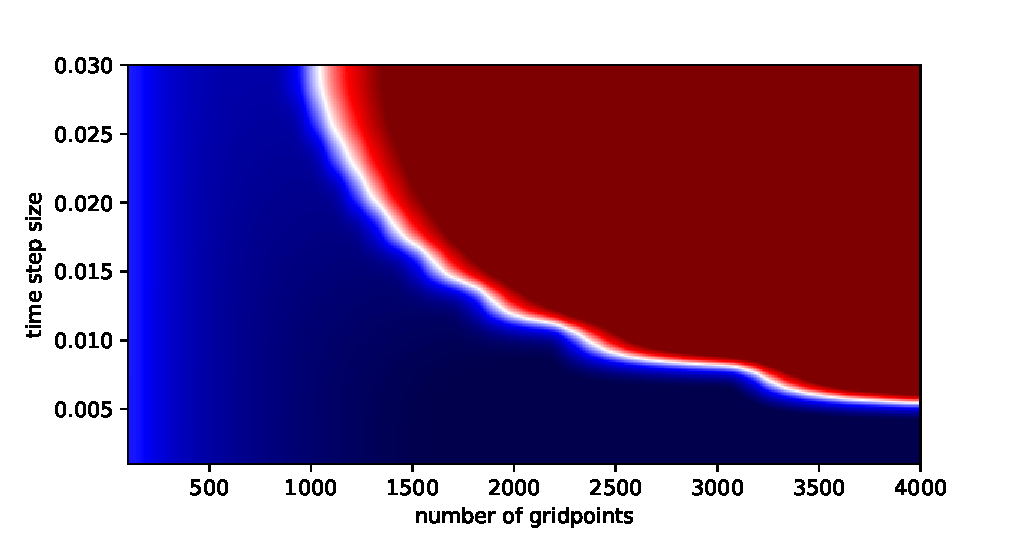
\includegraphics[width=1.2\textwidth]{figures/heatmap_wave_eq_step_size_numgridpoints.pdf}}
    \caption{Heatmap of log(Error) for wave equation over different spacial and temporal resolutions}
    \label{fig:heatmap_wave_eq_step_size_numgridpoints}
	\small
The white stripe represents the area where the log-error is 0, i.e. the actual error is 1.
The red area represents the area where the log-error is positive (can reach values up to $150$), i.e. large.
The blue area represents the area where the log-error is negative (can reach values down to $-20$), i.e. small.
\end{figure}

%$frac{dx}{dt}=\frac{t}{t^2+1}$, which has the solution $x_0 + 0.5\text{ln}(t^2+1)$.



%a time-invariant differential equation with only one variable (i.e. no spacial resolution), then a time-variant differential equation with no spacial resolution, and finally against a differential.
%First off, to verify the implementation, the RK-Integrators were used to solve a differential equation without any spacial resolution, but with temporal variance.
%$\frac{dx}{dt}=\frac{t}{t^2+1}$
%with solution $x_0 + 0.5\text{ln}(t^2+1)$.

%explain how time-step-size and grid-size have to change together, and show trough examples how accuracy changes depending on the choice of these two parameters (maybe a heatmap with x-axis = time-step-size, y-axis=grid-size, color=accuracy after simulation time T?)
%\subsubsection{Exponential Integrators}
%showcase how accuracy stays constant independent of time-step-size (for linear systems)\\
%give a small example of simulating a non-linear system by linearization around the current state


\section{Study of Errors in Implementation of NSE}
In this section the two implementations of the NSE are analyzed.
As no benchmarking systems for testing the vertical of the non-hydrostatic NSE-equations in isolation exist, true verification of the implementation is not possible.
Instead, four tests will be considered:
\begin{itemize}
\item comparison with a stationary solution
\item comparison of stationary solution with real world measurements
\item energy conservation
\item comparison of the two implementations to one another
\end{itemize}

\subsection{Comparison with Stationary Solution}
To find a stationary solution for the non-hydrostatic NSE, all time-derivatives have to be set to zero:
\begin{align}
\frac{\partial w}{\partial t} =0&= -g\left(1 - \frac{\partial p}{\partial s}\left(\frac{\partial \pi}{\partial s}\right)^{-1}\right)\label{stat_dw_dt} \\
\frac{\partial \text{ln}p}{\partial t}=0 &= \frac{g}{1- \frac{R}{C_p}} \frac{p}{RT}\left(\frac{\partial \pi}{\partial s}\right)^{-1} \frac{\partial w}{\partial s}\label{stat_dlnp_dt}\\
\frac{\partial T}{\partial t} =0&= \frac{RT}{C_p}\frac{\partial \text{ln}p}{\partial t}\label{stat_dT_dt}
\end{align}
The first equation \ref{stat_dw_dt} yields the following identity for pressure:
\begin{align*}
\frac{\partial p}{\partial s}=\left(\frac{\partial \pi}{\partial s}\right)\\
\Rightarrow p(s)=\pi (s) + p_0
\end{align*}
The second equation \ref{stat_dlnp_dt} is requires one of the elements in the denominator to equal zero.
As neither $g$, $p$, nor $\left(\frac{\partial \pi}{\partial s}\right)^{-1}$ can be zero, the only possible option is that $\frac{\partial w}{\partial s}=0$, i.e. $w(s)=w_0 \forall s$.
Due to the boundary conditions, at the bottom of the atmosphere $w(1)=0$, so $w(s)=w_0 \forall s$.\\
The last equation \ref{stat_dT_dt} yields no information, because the right hand side is already zero, due to $\frac{\partial \text{ln}p}{\partial t}=0$.
This means $T$ can be chosen freely, e.g. $T=273K$.\\
Using this stationary solution to define the initial state of the system, the integrator is expected not to change the system state.
This is reflected by both implementations as can be seen in Fig. 

\begin{figure}[!h]
	\makebox[\textwidth]{ 
  		 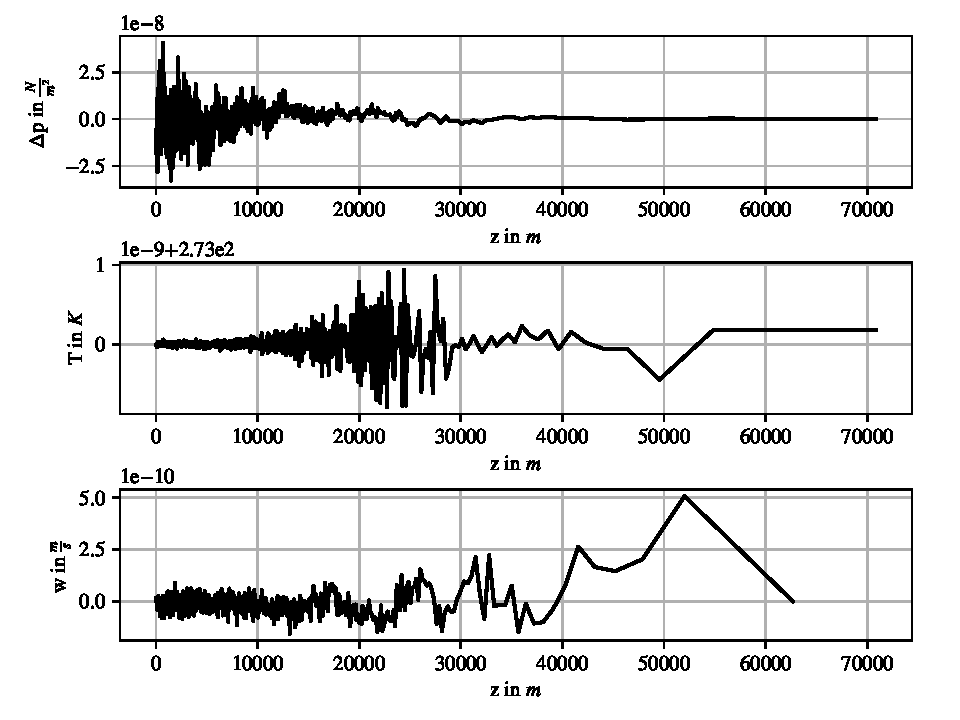
\includegraphics[width=1.2\textwidth]{figures/lorenz_240s_stat.pdf}}
    \caption{Error (deviation from stationary solution) made using RK4, time-step-size $2.5ms$, and $1000$ grid points, after $240s$ of simulation time}
    \label{fig:lorenz_stat_err}
\end{figure}

%In this section the effects (all?) possible choices of simplifications, integrators etc. is analyzed.\\
%To this end we introduce different ways of measuring errors, i.e. different norms, and use them to measure the difference between different simulations.

%\subsection{Simplifications to the Navier Stokes Equations} % effects of simplifications
%have one simulation without simplifications run with high precision (RK4 with tiny step-sizes and high grid resolution), and compare that to simulations using high precision with simplifications.

\subsection{Grid Discretizations}% grid discretizations
Quantify the difference between the two different grids.
How do we really know which one is better?
Find ways to quantify which one is more accurate?